\documentclass[11pt, oneside, reqno]{amsart}
\usepackage{fullpage}
\usepackage{amssymb,latexsym,amsmath,verbatim,layout,hyperref,amsthm,color,graphicx,mdframed,tikz,geometry,inputenc}  
\numberwithin{equation}{section}
\usepackage[T1]{fontenc}
%\usepackage[light,math]{anttor}
\usepackage {mathrsfs}
%package for good looking widehat
\usepackage{hyperref}
\usepackage{cleveref}
\usepackage{scalerel}

\makeatletter
\newcommand\makebig[2]{%
  \@xp\newcommand\@xp*\csname#1\endcsname{\bBigg@{#2}}%
  \@xp\newcommand\@xp*\csname#1l\endcsname{\@xp\mathopen\csname#1\endcsname}%
  \@xp\newcommand\@xp*\csname#1r\endcsname{\@xp\mathclose\csname#1\endcsname}%
}
\makeatother

\makebig{biggg} {3.0}
\makebig{Biggg} {3.5}
\makebig{bigggg}{4.0}
\makebig{Bigggg}{4.5}            
% AMS Theorems  
\theoremstyle{plain}% default
%\newtheorem{name}[counter]{text}[section]
\newtheorem{thm}{Theorem}[section]
\newtheorem{lem}[thm]{Lemma}
\newtheorem{prop}[thm]{Proposition}
\newtheorem{q}{Question}
\newtheorem*{ans}{Answer}
\newtheorem*{cor}{Corollary}


\theoremstyle{definition}
\newtheorem{defn}[thm]{Definition}
\newtheorem{conj}[thm]{Conjecture}
\newtheorem{exmp}[thm]{Example}


\theoremstyle{remark}
\newtheorem*{rmk}{Remark}
\newtheorem*{note}{Note}
\newtheorem{case}{Case}
\newtheorem{ex}{Exercise}
\newtheorem{eg}{Example}
\usepackage{hyperref}
\def\ci{\perp\!\!\!\perp}
\newcommand*{\bigchi}{\mbox{\Large$\chi$}} 
\renewcommand{\vec}[1]{\mathbf{#1}}


\newcommand{\e}{\mathbf{e}} 
    

\newcommand{\vgrad}{\mathbf{\nabla}}     
\newcommand{\vlap}{\mathbf{\Delta}}     
\newcommand{\sph}{\mathbb{S}}
%	x=  x,\quad  u,\quad \vgrad,\quad \vlap,\quad \sph
\newcommand{\R}{\mathbb{R}}
\renewcommand{\P}{\mathbb{P}}
\newcommand{\E}{\mathbb{E}}
\newcommand{\N}{\mathbb{N}}
\newcommand{\F}{\mathbb{F}}
\newcommand{\s}{\mathfrak{s}}
\newcommand{\A}{\mathcal{A}}

%\newcommand{\mbpRectIntensity}{\hat{\xi}^{\sqbullet}}

%geometry
\newcommand{\rectangle}{\tikz \fill [black] (0.1, 0.1) rectangle (0.2,0.2);}
\newcommand{\trapezoid}{\tikz \fill [black] (0.1, 0.2) -- (0.2,0.3) -- (0.3,0.3) -- (0.3,0.2) -- (0.1,0.2);}


\title{Power flow analysis
}


\author{Leanne Dong}

\date{\today}
\begin{document}
	\maketitle

\section{Introduction}
	Power flow analysis is a fundamental study discussed in any power system analysis textbook. The objective is to calculate the voltages (magnotude and angle) for a given load, generation and network condition. Once voltages are known for all buses, line flow and losses can be calculated. The starting point of solving power flow problem is to identify the known and unknown variables in the system. Based on these variables, buses are classified into three types: slack, generation (PV) and load buses (PQ). To recap Khaled's note, the slack bus is required to provide the mimatch between scheduled generation and total system load including losses and total generation. The slack bus is monthly considered as the reference bus because both voltage magnitude and angles are specified. The rest of generator buses are called regulated or PV buses as the net real power is specified and voltage magnitude is regulated. Most of the buses in practical power systems are load buses, the so-called PQ buses, since both net real and reactive power loads are specified.

For PQ buses, boh voltage magnitudes and angles are unknown, whereas for PV buses, only the voltage angle is unknown. As both voltage magnitudes and angles are specified for the Slack bus, there are no variables need to be solved. In a system with $n$ buses and $g$ generators, there are $2(n-1)-(g-1)$ unknowns. To solve these unknowns, real and reactive power balance equations are used. To write these equations, we need to model the transmission network using the admittance matrix ($Y$-bus)
In this note, I will mainly focus on the computation
of Jacobian matrix for Newton Raphson method.

\section{Admittance matrix and power flow equation}
\begin{align}
	A = \begin{bmatrix} 
	    Y_{11} & \dots & Y_{1n} \\
	    \vdots & \ddots & \\
	    a_{n1} & \dots & a_{nn} 
	    \end{bmatrix}
\end{align}
The values of diagonal elements $(Y_{ii})$ are equal to the sum of the admittances connected to bus $i$. The off-diagonal element $(Y_{ij})$ are equal to the negative of the admittance connecting the two buses $i$ and $j$. It is worth noting that with large system, $Y$-bus is a sparse matrix.
   \begin{align}
   	Y_{ii}&=\sum^n_{\substack{j=0 \\ j\neq i}}y_{ij}\\
	Y_{ij}&=Y_{ji}=-y_{ij}
   \end{align}
The net injected power at any bus can be calculated using the bus voltage ($V_i$), neighboring bus voltage $(V_j)$, and the admittances between the bus and its neighboring buses $(y_{ij})$ is
\begin{align*}
	I_i &= V_i y_{i0}+(V_i-V_1)y_{i1}
	+(V_i-V_2)y_{i2}+\cdots+(V_i-V_j)y_{ij}
\end{align*}
Rearranging the elements as function of voltages, the current equation becomes as follows:
\begin{align*}
	I_i&=V_i(y_{i0}+y_{i1}+y_{i2}+\cdots+y_{ij})-V_1 y_{i1} - V_2 y_{i2} - \cdots - V_j y_{ij}
\end{align*}


%\begin{align*}
\[
	I_i=V_i\sum_{\substack{j=0 \\ j\neq i}}y_{ij}-\sum_{\substack{j=1 \\ j\neq i}}y_{ij}= V_i Y_{ii}+\sum_{j=1\\ j\neq i}Y_{ij}V_j
\]
%\end{align*}

The complex power equation at any bus can be written as follows:
\begin{align*}
	S_i=P_i+jQ_1=V_i I^*_i
\end{align*}
or
\begin{align*}
	S^*_i=P_i-jQ_1=V^*_i I_i
\end{align*}
The complex power equation at any bus can be written as follows:
Substitututing the expression on the current in $S^*_i$ equation results in the following formula:

\[
	S^*_i = V^*_i\left(V_i\sum_{\substack{j=0 \\ j\neq i}}y_{ij}-\sum_{\substack{j=1 \\ j\neq i}}y_{ij}\right)
	= V^*_i\left(V_i Y_{ii}+\sum_{j=1\\ j\neq i}Y_{ij}V_j\right)
\]

Real and reactive power can be calculated from the following equations:
\[
	P_i=\text{Re}\Biggggl\{V^*_i\left(V_i\sum_{\substack{j=0 \\ j\neq i}}y_{ij}-\sum_{\substack{j=1 \\ j\neq i}}y_{ij}V_j\right)\Biggggr\}=\text{Re}\Biggggl\{V^*_i\left(V_i Y_{ii}+\sum_{j=1\\ j\neq i}Y_{ij}V_j\right)\Biggggr\}
\]
	      
\[	
Q_i=-\text{Im}\Biggggl\{V^*_i\left(V_i\sum_{\substack{j=0 \\ j\neq i}}y_{ij}-\sum_{\substack{j=1 \\ j\neq i}}y_{ij}V_j\right)\Biggggr\}=-\text{Im}\Biggggl\{V^*_i\left(V_i Y_{ii}+\sum_{j=1\\ j\neq i}Y_{ij}V_j\right)\Biggggr\}
\]
or simply
\begin{align}
	P_i&=\sum^n_{j=1}|V_i||V_j||Y_{ij}|\cos(\theta_{ij}-\delta_i+\delta_j)\\
	Q_i&=-\sum^n_{j=1}|V_i||V_j||Y_{ij}|\sin(\theta_{ij}-\delta_i+\delta_j)
\end{align}
And the current ($I_i$) can be written as a function of the power as follows:
\[
 \frac{P_i-jQ_i}{V^*_i}=V_i\sum_{\substack{j=0 \\ j\neq i}}y_{ij}-\sum_{\substack{j=1 \\ j\neq i}}y_{ij}V_j = V_i Y_{ii}+\sum_{j=1\\ j\neq i}Y_{ij}V_j
\]
\begin{figure}[!ht]
  \centering
  \begin{minipage}[b]{0.5\textwidth}
    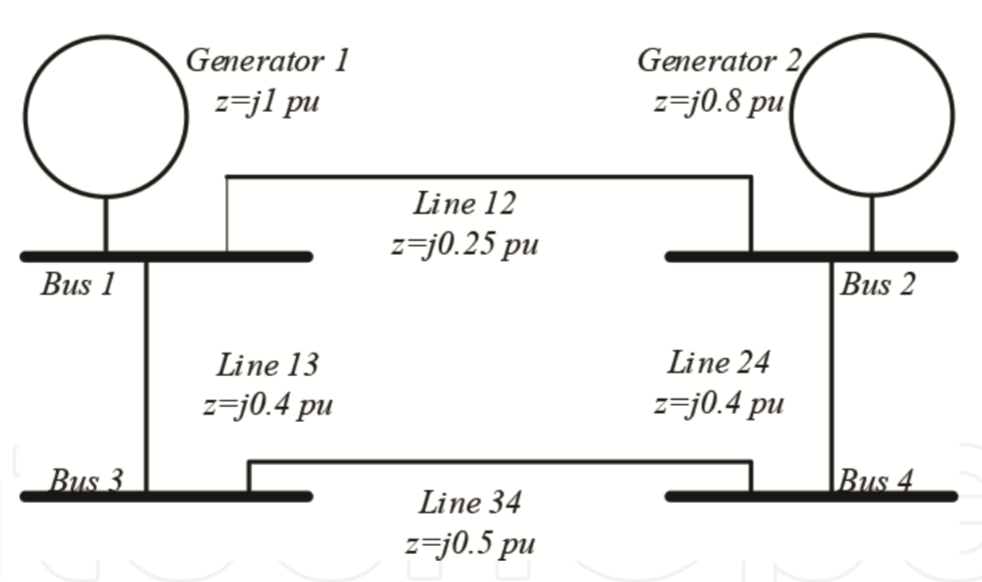
\includegraphics[width=\textwidth]{fig2.png}
    \caption[figure 2]{Impedance diagram}
  \end{minipage}
  \hfill
  \begin{minipage}[b]{0.5\textwidth}
    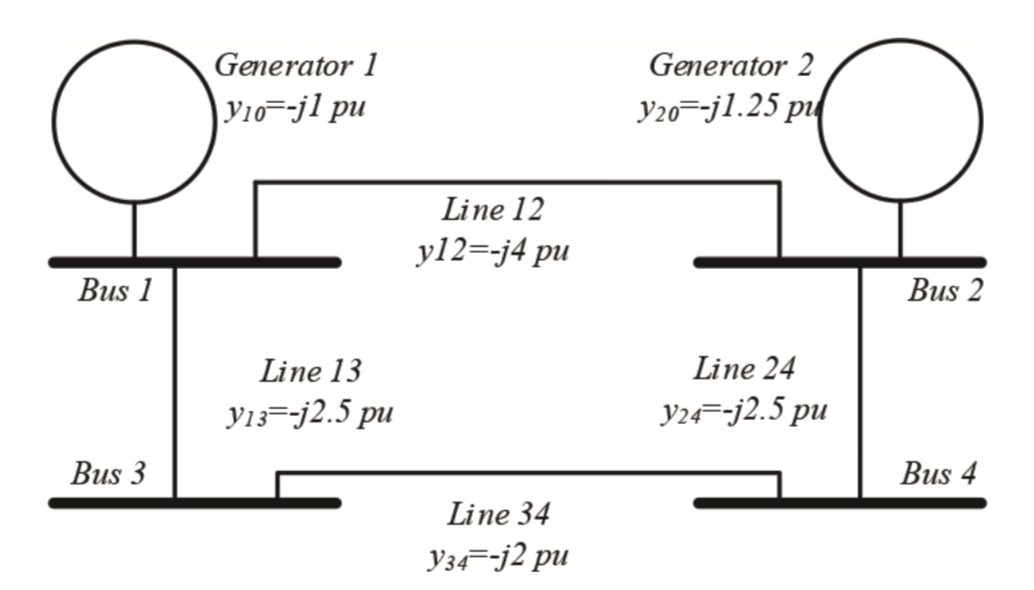
\includegraphics[width=\textwidth]{fig3.png}
    \caption[figure 3]{Admittance diagram}
  \end{minipage}
\end{figure}

\section{Newton-Raphson technique}

\end{document}